% Name: Angles in the same segment
% Description: Inscribed angles ACB and ADB stand on the same chord AB from the same side, so they are equal.
% Tags: circle theorem, inscribed angle, chord, same segment

\usetikzlibrary{angles, quotes}

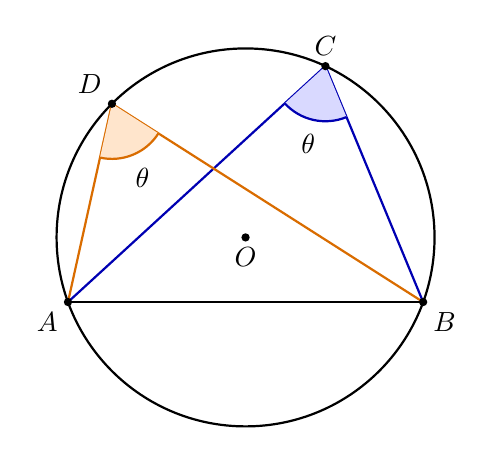
\begin{tikzpicture}[thick]
  % Arc AB (not containing C and D) spans 340 - 200 = 140 degrees, so each inscribed angle is 70 degrees
  \coordinate[label=below left:$A$] (A) at (200:2.4);
  \coordinate[label=below right:$B$] (B) at (340:2.4);
  \coordinate[label=above:$C$] (C) at (65:2.4);
  \coordinate[label=above left:$D$] (D) at (135:2.4);
  \fill (0,0) circle (1.5pt) node[below] {$O$};
  \draw (0,0) circle (2.4);
  \draw (A) -- (B);
  \draw[blue!70!black] (A) -- (C) -- (B);
  \draw[orange!85!black] (A) -- (D) -- (B);
  \pic[draw=blue!70!black, fill=blue!15, angle radius=7mm, angle eccentricity=1.45, "$\theta$"] {angle=A--C--B};
  \pic[draw=orange!85!black, fill=orange!20, angle radius=7mm, angle eccentricity=1.45, "$\theta$"] {angle=A--D--B};
  \foreach \p in {A, B, C, D} \fill (\p) circle (1.5pt);
\end{tikzpicture}
